
\documentclass[twocolumn,10ptr]{article}

\usepackage[linguistics]{forest}
\usepackage{cancel}
\usepackage{url}
\let\oldurl\url

\usepackage{tikz}
\usetikzlibrary{positioning,shapes,shadows,arrows,arrows.meta}
\newcommand*{\less}{\textless}
\newcommand*{\more}{\textgreater}
\usepackage{listings}
\usepackage{color}

\definecolor{dkgreen}{rgb}{0,0.6,0}
\definecolor{gray}{rgb}{0.5,0.5,0.5}
\definecolor{lightgray}{rgb}{0.9,0.9,0.9}
\definecolor{mauve}{rgb}{0.58,0,0.82}

\lstset{frame=tb,
	language=Java,
	aboveskip=3mm,
	belowskip=3mm,
	showstringspaces=false,
	columns=flexible,
	basicstyle={\tiny\ttfamily},
	numbers=none,
	numberstyle=\tiny\color{gray},
	keywordstyle=\color{blue},
	commentstyle=\color{dkgreen},
	stringstyle=\color{mauve},
	backgroundcolor=\color{lightgray},
	breaklines=false,
	breakatwhitespace=false,
	tabsize=2,
}

\author{Miguel Lemos}
\date{\today}
\title{Compilation Techniques First Assignment}

\begin{document}
	
	\twocolumn
	\setlength{\columnsep}{20pt}
	\maketitle
	
	\begin{abstract}
		As the first assignment of the Compilation Techniques course directed by the professor Maximiliano Andr\'{e}s Eschoyez a symbol table for the C language was implemented, using JAVA and the ANTLR Netbeans plugin.
	\end{abstract}
	
	
	
	\section{Formal Grammar}
	In formal language theory, a grammar (when the context is not given, often called a formal grammar for clarity) is a set of production rules for strings in a formal language. The rules describe how to form strings from the language's alphabet that are valid according to the language's syntax. A grammar does not describe the meaning of the strings or what can be done with them in whatever context, only their form.
	[1]
	
	
	
	\section{Lexicon}
	As in usual in formal grammars, we will suppose that we have some finite \textsc{BaseExp} of basic expressions. For our purposes, \textsc{BaseExp}  can be taken to be a finite subset of \cancel{English words}  C valid expressions. A \textit{lexicon} is then simply taken to be a relation between basic expressions and pairs consisting of syntactic categories and semantic objects of the appropiate types.
	More formally, a \textit{lexicon} is a relation:
	
	(1) \textsc{ lex} \( \subseteq \)  \textsc{ BasExp} (\textsc{Cat}(\textsc{BasCat})\(\times\) D)
	subject to the semantic well-typing constraint that:
	
	(2) if (e, ...\( \alpha \), f) \( \in \)   \textsc{ lex} is a lexical entry then f is an element of the domain D\textsubscript{\(\tau \)(\( \alpha \))\(\cdot\)} [2]
	
	With \textit{lexicon} defined, a \textit{lexeme} is defined in computer science differently than  \textit{lexeme}  in linguistics. A  \textit{lexeme}  in computer science roughly corresponds to what might be termed a word in linguistics (the term word in computer science has a different meaning than word in linguistics), although in some cases it may be more similar to a morpheme.
	
	A  \textit{lexeme}  is a string of characters which forms a syntactic unit.[3]
	
	Some authors term this a  \textit{token} , using 'token' interchangeably to represent (a) the string being tokenized, and (b) the token data structure resulting from putting this string through the tokenization process.[4][5]
	
	A \textit{token}  or \textit{lexical token}  is a structure representing a lexeme that explicitly indicates its categorization for the purpose of parsing.[6] A category of tokens is what might be termed a part-of-speech in linguistics. Examples of token categories may include identifier and integer literal, although the set of token categories differ in different programming languages. The process of forming tokens from an input stream of characters is called tokenization. Consider this expression in the programming language C:
	
	sum = 3 + 2;
	
	Tokenized and represented by the following table:
	
	
	\begin{center}
		\begin{tabular}{||c c||} 
			\hline
			Lexeme & Token Category\\ [0.5ex] 
			\hline\hline
			sum	&	Identifier  \\ 
			\hline
			=	&	Assignment operator  \\ 
			\hline
			3	&	Integer literal  \\ 
			\hline
			+	&	Addition operator  \\ 
			\hline
			2	&	Integer literal  \\ 
			\hline
			;	&	End of statement  \\ [1ex] 
			\hline
		\end{tabular}
	\end{center}
	
	
	
	\section{Using ANTLR for Lexical Analisis}
	Let lexical analysis be the extraction of individual words or lexemes from an input stream of symbols and passing corresponding tokens back to the parser: the use of ANTLR provided the tools to process code and develop a lexical grammar, for it to be used in lexical analysis.\\\\
	Here are some of the regular expressions used, in the correct ANTLR sintax:\\
	
	(3) LOGIC\_OP : '\&\&'\(\mid\)'\(\mid\)\(\mid\)'\(\mid\)'!'; \\
	
	(4)  DATA\_TYPE : 'int'\(\mid\)'float'\(\mid\)'char';\\
	
	(5)  IDENTIFICATOR: (LETTER\(\mid\)DIGIT)+;\\
	
	Where some patterns can be appreciated: The Lexers must be written in all-caps, and can be anidated, like is the case with (5), which uses two lexers of lower precedence.
	On the topic of precendence: Precedence is used to avoid ambiguity:\\
	
	
	(6)  INT : (0..9)+;\\
	
	(7)  FLOAT : INT '.' INT';\\
	
	(8)  DIGIT : (INT\(\mid\)FLOAT)';\\
	
	ANTLR would have to choose, when being faced with an integer, between INT and DIGIT. And it would do so by the order they are written. where the higher they are, the higher the precedence over the others. This way (6) would always win over (6). Which is the opposite of what would happen if they were written like this:\\
	
	
	(7)  FLOAT : INT '.' INT';\\
	
	(8)  DIGIT : (INT\(\mid\)FLOAT)';\\
	
	(6)  INT : (0..9)+;\\
	
	With this in mind, (5) would have precedence over LETTER and DIGIT tokens. Each time a LETTER or a DIGIT was found, it would be treated as an IDENTIFICATOR.
	To avoid this, and preserve the precedence of the used tokens, a syntax rule should be used, not a lexer one. This was done in the case of the DIGIT rule.\\
	
	(9)  digit : INT\(\mid\)FLOAT;\\
	
	where:\\
	
	(10) for\_loop :  'for' '(' ID (EQUAL INT)? ';' comparation ';' assignation ')' (code\_block\(\mid\)stat);\\
	
	would guarantee that no type other than (6) was used inside a for loop as index.:\\
	
	In my compiler I supposed no floating point digits would be used inside of the for loop. I have been informed since that C allows for floats to be used inside for loops conditions, but the case remains:
	If it was the case that you wanted to specify a token of low precedence to be used, if you wanted not to let the index of a for loop to be DIGIT but only for it to be INT, then the figures (9) and (10) would provide the desired functionality.\\
	
	With that said, it seems like the following figure would actually be more representative of a valid C syntax.\\
	
	(11) for\_loop :  'for' '(' ID (EQUAL digit)? ';' comparation ';' assignation ')' (code\_block\(\mid\)stat);\\
	
	The opposite situation of this is when a token has a null precedence, by design. And ANTLR observes that possibility, having the \textit{fragment} keyword to use when a token is never going to be used other than as a part of composed ones.
	
	Finally it must be observed that no lexer rule is recursive, because that it is not a property supported by regular expressions. This feature is left for the syntax rules, as follows.
	
	\section{Recursive syntax}
	The composition of lexer rules into high order functions allows for recursion, and with recursion is gained the necessary expressivity needed to represent all of the possible combinations  in the language, be they computer or natural. A CFG is created, which is higher in the Chomsky hierarchy for relative expressiveness than regular expressions, nondeterministic finite automatons and regular grammars.[6] 
	
	\section{ Abstract Sintax Tree}
	An \textsc{Abstract Sintax Tree} can be implemented as a stack of\textit{ scopes}, starting from the global one. As an example, each start of a function is the start of a scope. But a local variable can also be created inside a conditioned block of code, where it cannot be accesed outside of it. At the end a generalization can be made where it is the braces that define the starts and the ends of scopes.
	Now what is a\textit{ scope}? A\textsc{ Scope} is a dictionary of identificators, used to identify the variables.
	And what happens if a variable belongs to a higher scope, and is used on a lower scope, where it is not registered? 
	
	To satisfy this problem, scopes must have a jerarchical structure, where they store a reference to the scope directly higher to them, until the scope is global and has null for a reference. A \textit{ tree} is then formed, because many lower scopes can share a parent scope.
	
	\section{ Running the AST}
	From running the implementation of the AST a problem was found: The variables declarated inside of the function parameters were not being taken into account during the tree walk, where a visitor object was supposed to push the scopes and their identificators. And the reason for it was discovered to be that in the created grammar, function parameters were not supposed to contain variable\_declarations inside of them. Where as seen in the figure 12, the only difference among the two sintax rules are that parametersList allows for type only declarations, while a variable must have an identificator.\\
	
	
	(12) parametersList : VALID\_C\_TYPES
	
	\ \ \ \ \ \ \ \ \ \ \ \      \(\mid\) VALID\_C\_TYPES ID
	
	\ \ \ \ \ \ \ \ \ \ \ \ \ \ \    \(\mid\) VALID\_C\_TYPES ID EQUAL to\_value
	
	\ \ \ \ \ \ \ \ \ \ \ \     \(\mid\) parametersList \textsc{\char13},\textsc{\char13}  parametersList
	
	\ \ \ \ \ \ \ \ \ \ \ \   	\(\mid\) ;\\
	
	
	variable\_declaration :  
	
	VALID\_C\_TYPES ( EQUAL to\_value)? (\textsc{\char13},\textsc{\char13} 
	
	VALID\_C\_TYPES? ID (EQUAL to\_value)?)*);\\
	
	With that being said, a fix came from merging the rules so that when a variable is identified inside of a function parameter list, it is parsed as a declaration of a variable.\\
	
	(13) parametersList : VALID\_C\_TYPES
	
	\ \ \ \ \ \ \ \ \ \ \ \      \(\mid\) variable\_declaration
	
	\ \ \ \ \ \ \ \ \ \ \ \   	\(\mid\) ;\\
	
	Now in order to support multiple comma separated VALID\_C\_TYPES the following rule could be implemented:\\
	
	(14) parametersList : 
	
	VALID\_C\_TYPES   (\textsc{\char13},\textsc{\char13} VALID\_C\_TYPES )*
	
	\ \ \ \ \ \ \ \ \ \ \ \      \(\mid\) variable\_declaration
	
	\ \ \ \ \ \ \ \ \ \ \ \   	\(\mid\) ;\\
	
	But we still have the problem of the combination of the two series, the one of VALID\_C\_TYPES and the one for identifiable variables.
	To achieve that recursion must be implemented:\\
	
	(15) parametersList :
	
	VALID\_C\_TYPES   (\textsc{\char13},\textsc{\char13} VALID\_C\_TYPES )*
	
	\ \ \ \ \ \ \ \ \ \ \ \      \(\mid\) variable\_declaration
	
	\ \ \ \ \ \ \ \ \ \ \ \      \(\mid\)  parametersList \textsc{\char13},\textsc{\char13}  parametersList
	
	\ \ \ \ \ \ \ \ \ \ \ \   	\(\mid\) ;\\
	
	Now there is a problem, a parameterList could be a series of empty terminals, and because we are using recursion we are technically supporting an infinite ammount of comma separated empty terminals as a function parameter list. To fix this, and all similar cases, we must avoid supporting recursivity on rules that support empty terminals.\\
	
	A final version of the parameterList sintax rule would be: (16)\\
	
	VALID\_C\_TYPES   (\textsc{\char13},\textsc{\char13} VALID\_C\_TYPES )*
	
	\ \ \ \ \ \ \ \ \ \ \ \      \(\mid\) variable\_declaration
	
	\ \ \ \ \ \ \ \ \ \ \ \      \(\mid\)  parametersList \textsc{\char13},\textsc{\char13}  parametersList;\\
	
	Where a function declaration, and prototype, can have either a parameterList, or an empty terminal, as valid parameters:\\
	
	(17)\\
	
	f\_d:VALID\_C\_TYPES ID \textsc{\char13}(\textsc{\char13} parametersList? \textsc{\char13})\textsc{\char13} code\_block ;\\
	
	f\_p:VALID\_C\_TYPES ID \textsc{\char13}(\textsc{\char13} parametersList? \textsc{\char13})\textsc{\char13}  ;\\
	
	
	\section{ Traversing the AST}
	As said, the AST can be thought of as a stack of scopes, where each contains the symbols that belong to them. In a hashset, preferably, for heuristic purposes. Now, a stack, by definition, contains a pop() function, that on call remove the last pushed element of the stack. This means that once the code is fully traversed, nothing of the AST data structure will remain stored. In order to preserve the information after compilation, a \textit{symbol table} must be created, to be looked up to. But more of that later. What use can be made of the traversing of the AST itself?\\
	
	CErrorException: Undeclared variable x at line 8\\
	
	By traversing the AST, higher scopes can be accesed from the lower, more recently added ones, so that variables that dont belong to the lower scopes and may belong to the higher scopes can be successfully identified as so, else a custom exception be handed to the user, stating the line and variable identificator.
	
	
	\section{ Creating a Symbols Table}
	Having a stack of scopes at hand, and knowing its existence is short-lived, the creation of a persistent storage becomes important. The current implementation of the scopes stack only stored the variables identificators. Now it should store the type and the value. It could store them all together; it would be suboptimal in the case of identificator-only queries. And so, a hashset that stores Symbols instead of only Strings, is needed, parallel to the old one. This hashset will store all of the symbols inside the Scope.\\
	
	(18)\\
	
	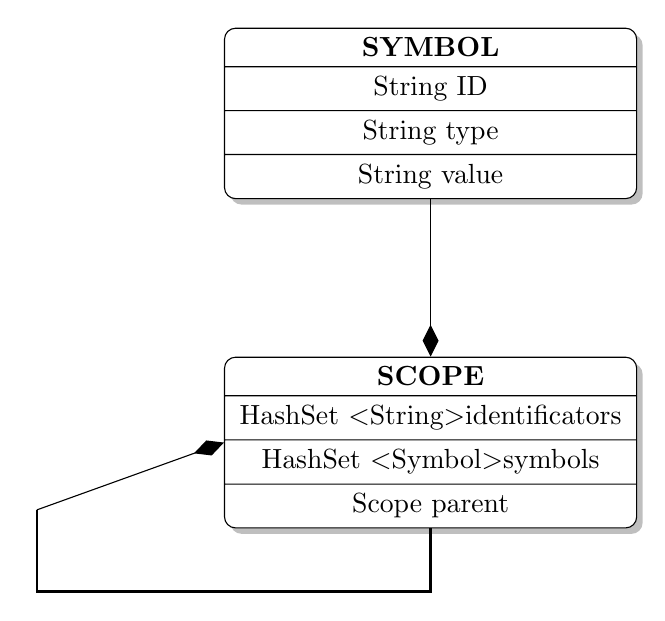
\begin{tikzpicture}[node distance=2cm]
	\tikzstyle{abstract}=[rectangle, draw=black, rounded corners, fill=white!40, drop shadow,
	text centered, anchor=north, text=black, text width=5cm]
	\tikzstyle{line}=[-, thick]
	\node (Symbol) [abstract, rectangle split, rectangle split parts=4]
	{
		\textbf{SYMBOL}
		\nodepart{second}String ID
		\nodepart{third}String type
		\nodepart{fourth}String value
	};        
	\node (Scope) [abstract, rectangle split, rectangle split parts=4,  below=of Symbol]
	{
		\textbf{SCOPE}
		\nodepart{second}HashSet \less String\more identificators
		\nodepart{third}HashSet \less Symbol\more symbols
		\nodepart{fourth}Scope parent
	};
	\node (auxiliar) at (-5,-6) {};
	
	\draw[{Diamond[fill=black,scale=2]}-{}] (Scope.north) -- ++(0,0.8) -| (Symbol.south);
	\draw[line] (Scope.south) -- ++(0,-0.8) -| (auxiliar.south);
	\draw[{}-{Diamond[fill=black,scale=2]}] (auxiliar.south) --  (Scope.west);
	\end{tikzpicture}
	\\
	\\
	
	
	Given that it is the Visitor object the one visiting the nodes and adquiring the information, it sounds reasonable for it to be owner of the two data structures composed of Scopes: \textit{temporal\_scopes}, the Stack, and \textit{symbolsTable}, the detailed and persistent HashSet, as seen in the figure (19).\\
	
	(19)\\
	
	
	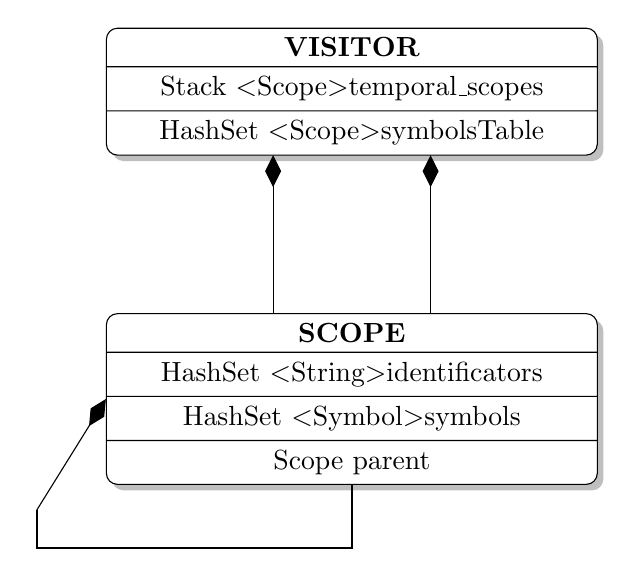
\begin{tikzpicture}[node distance=2cm]
	\tikzstyle{abstract}=[rectangle, draw=black, rounded corners, fill=white!40, drop shadow,
	text centered, anchor=north, text=black, text width=6cm]
	\tikzstyle{line}=[-, thick]
	\node (Visitor) [abstract, rectangle split, rectangle split parts=3]
	{
		\textbf{VISITOR}
		\nodepart{second}Stack \less Scope\more temporal\_scopes
		\nodepart{third}HashSet \less Scope\more symbolsTable
	};        
	\node (Scope) [abstract, rectangle split, rectangle split parts=4,  below=of Visitor]
	{
		\textbf{SCOPE}
		\nodepart{second}HashSet \less String\more identificators
		\nodepart{third}HashSet \less Symbol\more symbols
		\nodepart{fourth}Scope parent
	};
	\node (auxiliar) at (-4,-6) {};
	
	\draw[{}-{Diamond[fill=black,scale=2]}] (-1,-3.62) --  (-1,-1.62);
	\draw[{}-{Diamond[fill=black,scale=2]}] (1,-3.62) --  (1,-1.62);
	\draw[line] (Scope.south) -- ++(0,-0.8) -| (auxiliar.south);
	\draw[{}-{Diamond[fill=black,scale=2]}] (auxiliar.south) --  (Scope.west);
	\end{tikzpicture}
	\\
	
	This, while heavier on memory usage, allows for query-specific optimization, by giving ID queries priority over complete symbol ones.
	\section{Valid symbol initialization}
	A first semantic analysis check could be as simple as checking that identifiers are used appropiately within the program: C is capable of handling character literal on integer intialization, among other weird possible conversions, but a warning would not be out of place if a user would initialize integers using chars.\\
	
	Warning : Converting from int to char at line 1\\ \\
	Now there is a problem: ANTLR creates rules contexts like StringContext or any\_sintax\_ruleContext, for each of the sintax rules created in the grammar. It does not do so, however, for the lexer rules. And so the above warning is completely feasible using the current set of sintax rules, be them:\\
	
	string : \textsc{\char13}''\textsc{\char13}(ID\(\mid\)digit)+ \textsc{\char13}''\textsc{\char13} \(\mid\) \textsc{\char13}\textbackslash\textsc{\char13}\textsc{\char13}  (ID\(\mid\) DIGIT)+ \textsc{\char13}\textbackslash\textsc{\char13}\textsc{\char13};
	
	digit: INT \(\mid\) FLOAT;
	
	Because it can recognize that the type of a variable, in this case \textit{ int}, should not be initialized by a StringContext, which translated by a dictionary evaluates to \textit{char}.\\
	
	(20)
	\{  ''StringContext'' : ''char'' \}\\
	
	The problem begins when trying to check for floating point truncation. Then the dictionary has no use against the ambiguity of the digit sintax rule, suffering from key collision because the digit syntax rule can be either a float or an int.\\
	
	(21)
	\{  ''StringContext'' : ''char'',
	
	\ \ \ \ \ \ \ \ \ \   ''DigitContext'' : ''float'',
	
	\ \ \ \ \ \ \ \ \ \   ''DigitContext'' : ''int''
	
	\ \ \ \ \ \ \    \}\\
	
	Transforming the lexers INT and FLOAT into the sintax rules int and float made (22) possible.\\
	
	(22)
	\{  ''StringContext'' : ''char'',
	
	\ \ \ \ \ \ \ \ \ \   ''FloatContext'' : ''float'',
	
	\ \ \ \ \ \ \ \ \ \   ''IntContext'' : ''int'',  
	
	\ \ \ \ \ \ \    \}\\
	
	
	(23) var\_declaration : 
	
	\ \ \ \ \ \ \ \ \ \ \ \  VALID\_C\_TYPES ID (EQUAL to\_value)?
	
	\ \ \ \ \ \ \ \ \ \    (\textsc{\char13} ,\textsc{\char13}  VALID\_C\_TYPES? ID 
	
	\ \ \ \ \ \ \ \ \ \   (EQUAL to\_value)?)*;\\
	(24) to\_value : ID\(\mid\)digit\(\mid\)string\(\mid\)f\_c\(\mid\)math\_operator;\\
	(25) digit : int \(\mid\) float;\\
	
	So that when asking variable\_declaration(23) for the type VALID\_C\_TYPES evaluated to, this string, which can be \textsc{\char13}int\textsc{\char13}, \textsc{\char13}float\textsc{\char13} or \textsc{\char13}char\textsc{\char13} to name a few, can be successfully compared against the dictionary entry for the ruleContext to\_value was evaluated to. Say it was the float syntax rule, then the ruleContext would be named FloatContext, and the entry for FloatContext would resolve into  ''float'', which compared against  ''int'' returns false, and a warning is released.\\
	
	Warning : Converting from float to int at line 1\\
	
	
	
	
	\section{Flattening trees}
	In C, a function prototype, a function declaration, and a function call, all have parameters. The last replaces them with information, the second gives local names to that information to be used inside the function, and the first one can give the parameters names, or not. *See (16) for the parameter list and (16) for the function prototype rule.
	
	To avoid going back lets bring the figure 16: (16)\\
	
	VALID\_C\_TYPES   (\textsc{\char13},\textsc{\char13} VALID\_C\_TYPES )*
	
	\ \ \ \ \ \ \ \ \ \ \ \      \(\mid\) variable\_declaration
	
	\ \ \ \ \ \ \ \ \ \ \ \      \(\mid\)  parametersList \textsc{\char13},\textsc{\char13}  parametersList;\\
	
	Here it can be noted that a parameterList will not contain another parameterList inside while its parameters are all either a comma separated list of VALID\_C\_TYPES or a comma separated list of declarated variables, where the difference among them is that one is unnamed and the other one is.
	
	With this being said, an example could show the problem in detail:\\
	
	Let f\_p be a function prototype:\\
	
	f\_p(int, int, int a, int b, char);
	
	\newcommand*{\equal}{=}
	\newcommand*{\comma}{,}
	
	\begin{forest}
		[parameterList
		[parameterList
		[int]
		[int]
		]
		[parameterList
		[int a]
		[int b]
		]
		
		[parameterList
		[
		char
		]
		]
		
		]
		
	\end{forest}
	
	The problem starts when trying to get the list of parameters from the parameterList rule, where the data structure is not a list but a tree.
	
	\section{The imperative way}
	
	Thinking imperatively is a regular problem for developers when facing problems that can be solved with imperative solutions. Applying old algorithms to new problems seems like a reasonable solution.
	Here is how I adapted the BFS algorithm to my problem. 
	
	
	\begin{lstlisting}



List<String> Parameters = new ArrayList();
Queue<CParser.ParametersListContext> parametersContexts = new ArrayDeque<>();
parametersContexts.add(ctx.parametersList());

while (!parametersContexts.isEmpty()){
	//parameters can contain  parameters, so its important to get them all
	CParser.ParametersListContext currentParametersListContext = parametersContexts.poll();
	ParseTree parameterFirstChild = currentParametersListContext.children.get(0);
	try{
		Parameters.add(
		((CParser.Variable_declarationContext)parameterFirstChild).VALID_C_TYPES().stream()
		.map( n -> n.getText())
		.collect( Collectors.joining( "," ))
		);	
	}
	catch(java.lang.ClassCastException e){}
	
	try{
		Parameters.add(((org.antlr.v4.runtime.tree.TerminalNodeImpl)parameterFirstChild)
		.getParent().getText());	
	}
	catch(java.lang.ClassCastException e){}
	
	currentParametersListContext.children.forEach(child -> { 
		try{
			CParser.ParametersListContext nextParametersListContext =
				((CParser.ParametersListContext) child);
			parametersContexts.add(nextParametersListContext);
		}
		catch(java.lang.ClassCastException e){}
	});
}

List<String> flattenedParametersTypes = Arrays.asList(Parameters.toString().split(","));

	\end{lstlisting}
	
	It is to be noted that the resulting array is reversed.
	
	
	\section{The functional way}
	Now, if there is a correct way of flattening a tree-based data structure, it is probably functional. Here is how I did it, using Java 8 streams, flatMap, filters and  collectors.\\
	
	\begin{lstlisting}
	List<String> flattenedParametersTypes = ctx.parametersList().children.stream()
	
	.flatMap(enterRules::flattenParameters)
	.filter(string -> !string.isEmpty())
	.collect(Collectors.toList());
	
	flattenedParametersTypes =
	 Arrays.asList(
	   flattenedParametersTypes.toString().split(",")
	 ); 
	\end{lstlisting}
	
	\\It is to be noted that the resulting array is not reversed. \\
	
	Now if those were all the lines needed to perform the task, the functional way would have proven itself to be incredibly expressive. And it is, its just that the total ammount of lines is bigger than that because of the auxiliar function used. Which goes as follows:
	
		\begin{lstlisting}

public static Stream<String> flattenParameters(ParseTree parameterListParseTree) {
	Stream<String> stringStream = null;
	try{
		//this filters children from ruleF_pContext like the parentheses
		CParser.ParametersListContext parameterList =
			 ((CParser.ParametersListContext)parameterListParseTree);
		
		
		stringStream = Stream.concat(
		
		Stream.of(
			//At this point we can safely assume we are visiting every parameterList
			
			//but because ParameterLists contain ParameterList
			//we only want to work with the terminals, the ones 
			//that don't contain ParameterLists  
			
			((!parameterList.parametersList().isEmpty())? "":
				//and now we safely cast between the two remaining options:
				
				//is it just a list of TOKENS? 
				parameterList.children.get(0) instanceof
				 org.antlr.v4.runtime.tree.TerminalNodeImpl ? 
						parameterList.getText() 
						: 
				//or is it a variable declaration rule? 
				parameterList.children.get(0) instanceof
				 CParser.Variable_declarationContext ?
						((CParser.Variable_declarationContext)parameterList.children.get(0))
						.VALID_C_TYPES().stream()
								.map( n -> n.getText()                                                    
								)
								.collect( Collectors.joining( "," )) 
						: ""
				)
		
		), 
		parameterList.children.stream().flatMap((parameterListParameterList) ->
		 enterRules.flattenParameters(parameterListParameterList))); // recursion here
		
	}catch(java.lang.ClassCastException e){}
	
	return stringStream;
}
	\end{lstlisting}
	
	The final result of both implementations is an array that contains the types of the parameters in the way they are meant to be visualized, as a list: [int, int, int, char, char]

	
	
	
	
	
	
	
	\onecolumn
	\begin{thebibliography}{9}
		\bibitem{formalgrammar} 
		\url{https://en.wikipedia.org/wiki/Formal_grammar}
		\bibitem{lexicon} 
		page 173, "Formal Grammar: Theory and Implementation", by Robert Levine
		
		\bibitem{lexicon1} 
		page 111, "Compilers Principles, Techniques, \& Tools, 2nd Ed." (WorldCat) by Aho, Lam, Sethi and Ullman, as quoted in \url{https://stackoverflow.com/questions/14954721/what-is-the-difference-between-token-and-lexeme}  
		
		\bibitem{lexicon2} 
		Perl 5 Porters. "perlinterp: Perl 5 version 24.0 documentation". perldoc.perl.org - Official documentation for the Perl programming language. perldoc.perl.org. Retrieved 26 January 2017.
		
		\bibitem{lexicon3}
		Guy Coder (19 February 2013). "What is the difference between token and lexeme?". Stack Overflow. Stack Exchange Inc. Retrieved 26 January 2017.
		
		\bibitem{lexicon4}
		\url{https://en.wikipedia.org/wiki/Lexical_analysis}
		
		\bibitem{chomsky} 
		\url{https://en.wikipedia.org/wiki/Expressive_power_(computer_science)}
		
		
	\end{thebibliography}
	
	
	
	
	
\end{document}
Contact GitHub API Training Shop Blog About
© 2017 GitHub, Inc. Terms Privacy Security Status Help